In this chapter we will evaluate the architectures described in chapter \ref{chapter:architectures} with the method described in chapter \ref{chapter:design_of_experiments}. Some of them will additionally be evaluated with the implementation from chapter \ref{chapter:implementation}.







\section{Bandwidth}
When evaluating we are making some assumptions about bandwidth. Table \ref{tab:Bandwidth_latency} shows latency and bandwidth for different technologies. The WiFi bandwidths are based on data from CenturyLink\cite{noauthor_24_nodate}. The 4G and 5G bandwidths are real-world examples from 4g.co.uk\cite{noauthor_how_nodate}. The 4G latency are from ping tests, while the 5G latency are from Verizon\cite{noauthor_what_2020}.

\begin{table}[h!]
    \centering
    \begin{tabular}[c]{|c|c|c|}
        \hline
        Technology & Latency (ms) & Bandwidth (Mbps) \\
            &   &  Download/Upload \\
        \hline
        \hline
        Wifi (2.4GHz) & <=1 & 150/150  \\
        \hline
        Wifi (5GHz) & <=1 & 450/450  \\
        \hline
        4G & 30-65 & 42/25  \\
        \hline
        5G & 30 & 200/100  \\
        \hline
        Wired LAN & <=1 & 1000+  \\
        \hline
        WAN & 10-300+ & 1000+  \\
        \hline
        
        
    \end{tabular}
    \caption{Latency and bandwidth for different technologies.}
    \label{tab:Bandwidth_latency}
\end{table}
When doing calculations in this chapter, we will be using numbers from table \ref{tab:Bandwidth_latency}.









\section{Multi-Access Edge Computing}
MEC seeks to offload a reasonable amount of work. Therefore, we will not offload all the work, but rather test with several ratios of computation offloading. It is not always efficient to offload all the work. According to Mach and Becvar´s survey\cite{mach_mobile_2017}, we can divide offloading into three categories:
\begin{itemize}
    \item \textit{Local execution}, where all the work is done on the mobile device.
    \item \textit{Full offloading}, where we offload all work to server(s).
    \item \textit{Partial offloading}, where we offload some of the work, and do some local.
\end{itemize}
We will compare these three. We will also test different variations of Partial offloading. According to cpubenchmark\cite{noauthor_passmark_nodate}, flagship phones is about half as fast as a standard desktop CPU. We assume that we are dealing with below average CPU's cellphones, as most people do not have the flagship phone. We will test different strengths of the MEC Server. We assume that the data centre will have plenty of resources. In total, we want to do 10000 iterations spread over all the nodes.

\subsection{Local execution}
%lacking geographic location?
\begin{table}[h!]
    \centering
    \begin{tabular}[c]{|c|c|c|c|}
        \hline
        Node type & Limitation & Iterations & Time used (s) \\
        \hline
        \hline
        Local & 30 & 10000 & 333.6 \\
        \hline
    \end{tabular}
    \caption{Only local execution}
    \label{tab:MEC_local_execution}
\end{table}
Table \ref{tab:MEC_local_execution} shows the time used for local execution only.



\subsection{Full execution}
%spread out over more nodes
Here we offload all the work to the nodes. Since the Far node has more resources we let it do more of the work.
\begin{table}[h!]
    \centering
    \begin{tabular}[c]{|c|c|c|c|}
        \hline
        Node type & Limitation & Iterations & Time used (s)\\
        \hline
        \hline
        Local & 30 & 0 & 0 \\
        \hline
        Near & 100 & 2500 & 23.3 \\
        \hline
        Far & 300 & 7500 & 30.5 \\
        \hline
    \end{tabular}
    \caption{Full offloading execution}
    \label{tab:MEC_full_execution}
\end{table}

\begin{table}[h!]
    \centering
    \begin{tabular}[c]{|c|c|c|c|}
        \hline
        Node type & Limitation & Iterations & Time used (s)\\
        \hline
        \hline
        Local & 30 & 0 & 0 \\
        \hline
        Near & 100 & 2800 & 27.3 \\
        \hline
        Far & 300 & 7200 & 29.8 \\
        \hline
    \end{tabular}
    \caption{Full offloading execution with more balance}
    \label{tab:MEC_full_execution_balanced}
\end{table}

Table \ref{tab:MEC_full_execution} and \ref{tab:MEC_full_execution_balanced} shows time used when offloading work to nodes. However, here we only send the workload once, and it does not need to do any communication until the work is done.

\begin{table}[h!]
    \centering
    \begin{tabular}[c]{|c|c|c|c|c|}
        \hline
        Node type & Limitation & Iterations & RTT to Local (ms)& Time used (s)\\
        \hline
        \hline
        Local & 30 & 0 & 0 & 0 \\
        \hline
        Near & 100 & 2800 & 30 & 92.8 \\
        \hline
        Far & 300 & 7200 & 170 & 1304.8 \\
        \hline
    \end{tabular}
    \caption{Full offloading execution with communication between Local and Near/Far}
    \label{tab:MEC_full_execution_latency}
\end{table}

Table \ref{tab:MEC_full_execution_latency} shows how latency affects the work. We get a very big slowdown from when all is done locally. 

\begin{table}[h!]
    \centering
    \begin{tabular}[c]{|c|c|c|c|c|}
        \hline
        Node type & Limitation & Iterations & RTT to Local (ms)& Time used (s)\\
        \hline
        \hline
        Local & 30 & 0 & 0 & 0 \\
        \hline
        Near & 100 & 8500 & 30 & 279.3 \\
        \hline
        Far & 300 & 1500 & 170 & 267.9 \\
        \hline
    \end{tabular}
    \caption{Full offloading execution with communication and more balance in the nodes}
    \label{tab:MEC_full_execution_latency_balance}
\end{table}

Table \ref{tab:MEC_full_execution_latency_balance} shows a more balanced workload distribution. The Near node is doing significantly more work. Due to latency they use about the same time.

%TODO find out where they balance out. Finn en likning for det?
% planet7 og planet-70ms
% eksprementer med 5k totalt istedet for 10k
% Le














\subsection{Partial execution}
For partial execution, we want all nodes to work.
\begin{table}[h!]
    \centering
    \begin{tabular}[c]{|c|c|c|c|}
        \hline
        Node type & Limitation & Iterations & Time used (s)\\
        \hline
        \hline
        Local & 30 & 1000 & 33.0 \\
        \hline
        Near & 100 & 2000 & 19.5 \\
        \hline
        Far & 300 & 7000 & 30.6 \\
        \hline
    \end{tabular}
    \caption{Partial offloading execution}
    \label{tab:MEC_partial_execution}
\end{table}


\begin{table}[h!]
    \centering
    \begin{tabular}[c]{|c|c|c|c|}
        \hline
        Node type & Limitation & Iterations & Time used (s)\\
        \hline
        \hline
        Local & 30 & 850 & 28.1 \\
        \hline
        Near & 100 & 2700 & 26.5 \\
        \hline
        Far & 300 & 6450 & 29.1 \\
        \hline
    \end{tabular}
    \caption{Partial offloading execution with more balance}
    \label{tab:MEC_partial_execution_balanced}
\end{table}
Table \ref{tab:MEC_partial_execution} and \ref{tab:MEC_partial_execution_balanced} shows offloading with little overhead and no latency.






\begin{table}[h!]
    \centering
    \begin{tabular}[c]{|c|c|c|c|c|}
        \hline
        Node type & Limitation & Iterations & RTT to Local (ms)& Time used (s)\\
        \hline
        \hline
        Local & 30 & 850 & 0 & 28.1 \\
        \hline
        Near & 100 & 2700 & 30 & 86.0 \\
        \hline
        Far & 300 & 6450 & 170 & 1131.2 \\
        \hline
    \end{tabular}
    \caption{Partial offloading execution with communication between Local and Near/Far}
    \label{tab:MEC_partial_execution_latency}
\end{table}

Table \ref{tab:MEC_partial_execution_latency} shows how latency affects the work. We get a very big slowdown from when all is done locally. 

\begin{table}[h!]
    \centering
    \begin{tabular}[c]{|c|c|c|c|c|}
        \hline
        Node type & Limitation & Iterations & RTT to Local (ms)& Time used (s)\\
        \hline
        \hline
        Local & 30 & 4550 & 0 & 151.3  \\
        \hline
        Near & 100 & 4525 & 30 & 149.8 \\
        \hline
        Far & 300 & 925 & 170 & 163.0 \\
        \hline
    \end{tabular}
    \caption{Partial offloading execution with communication and more balance in the nodes}
    \label{tab:MEC_partial_execution_latency_balance}
\end{table}





\subsection{Comparison of results}
%nevn offloading. Vis stolpediagramm hvor en chunk av tiden er offloading. Vis også med N*latency?
\begin{figure}[t]
    \centering
    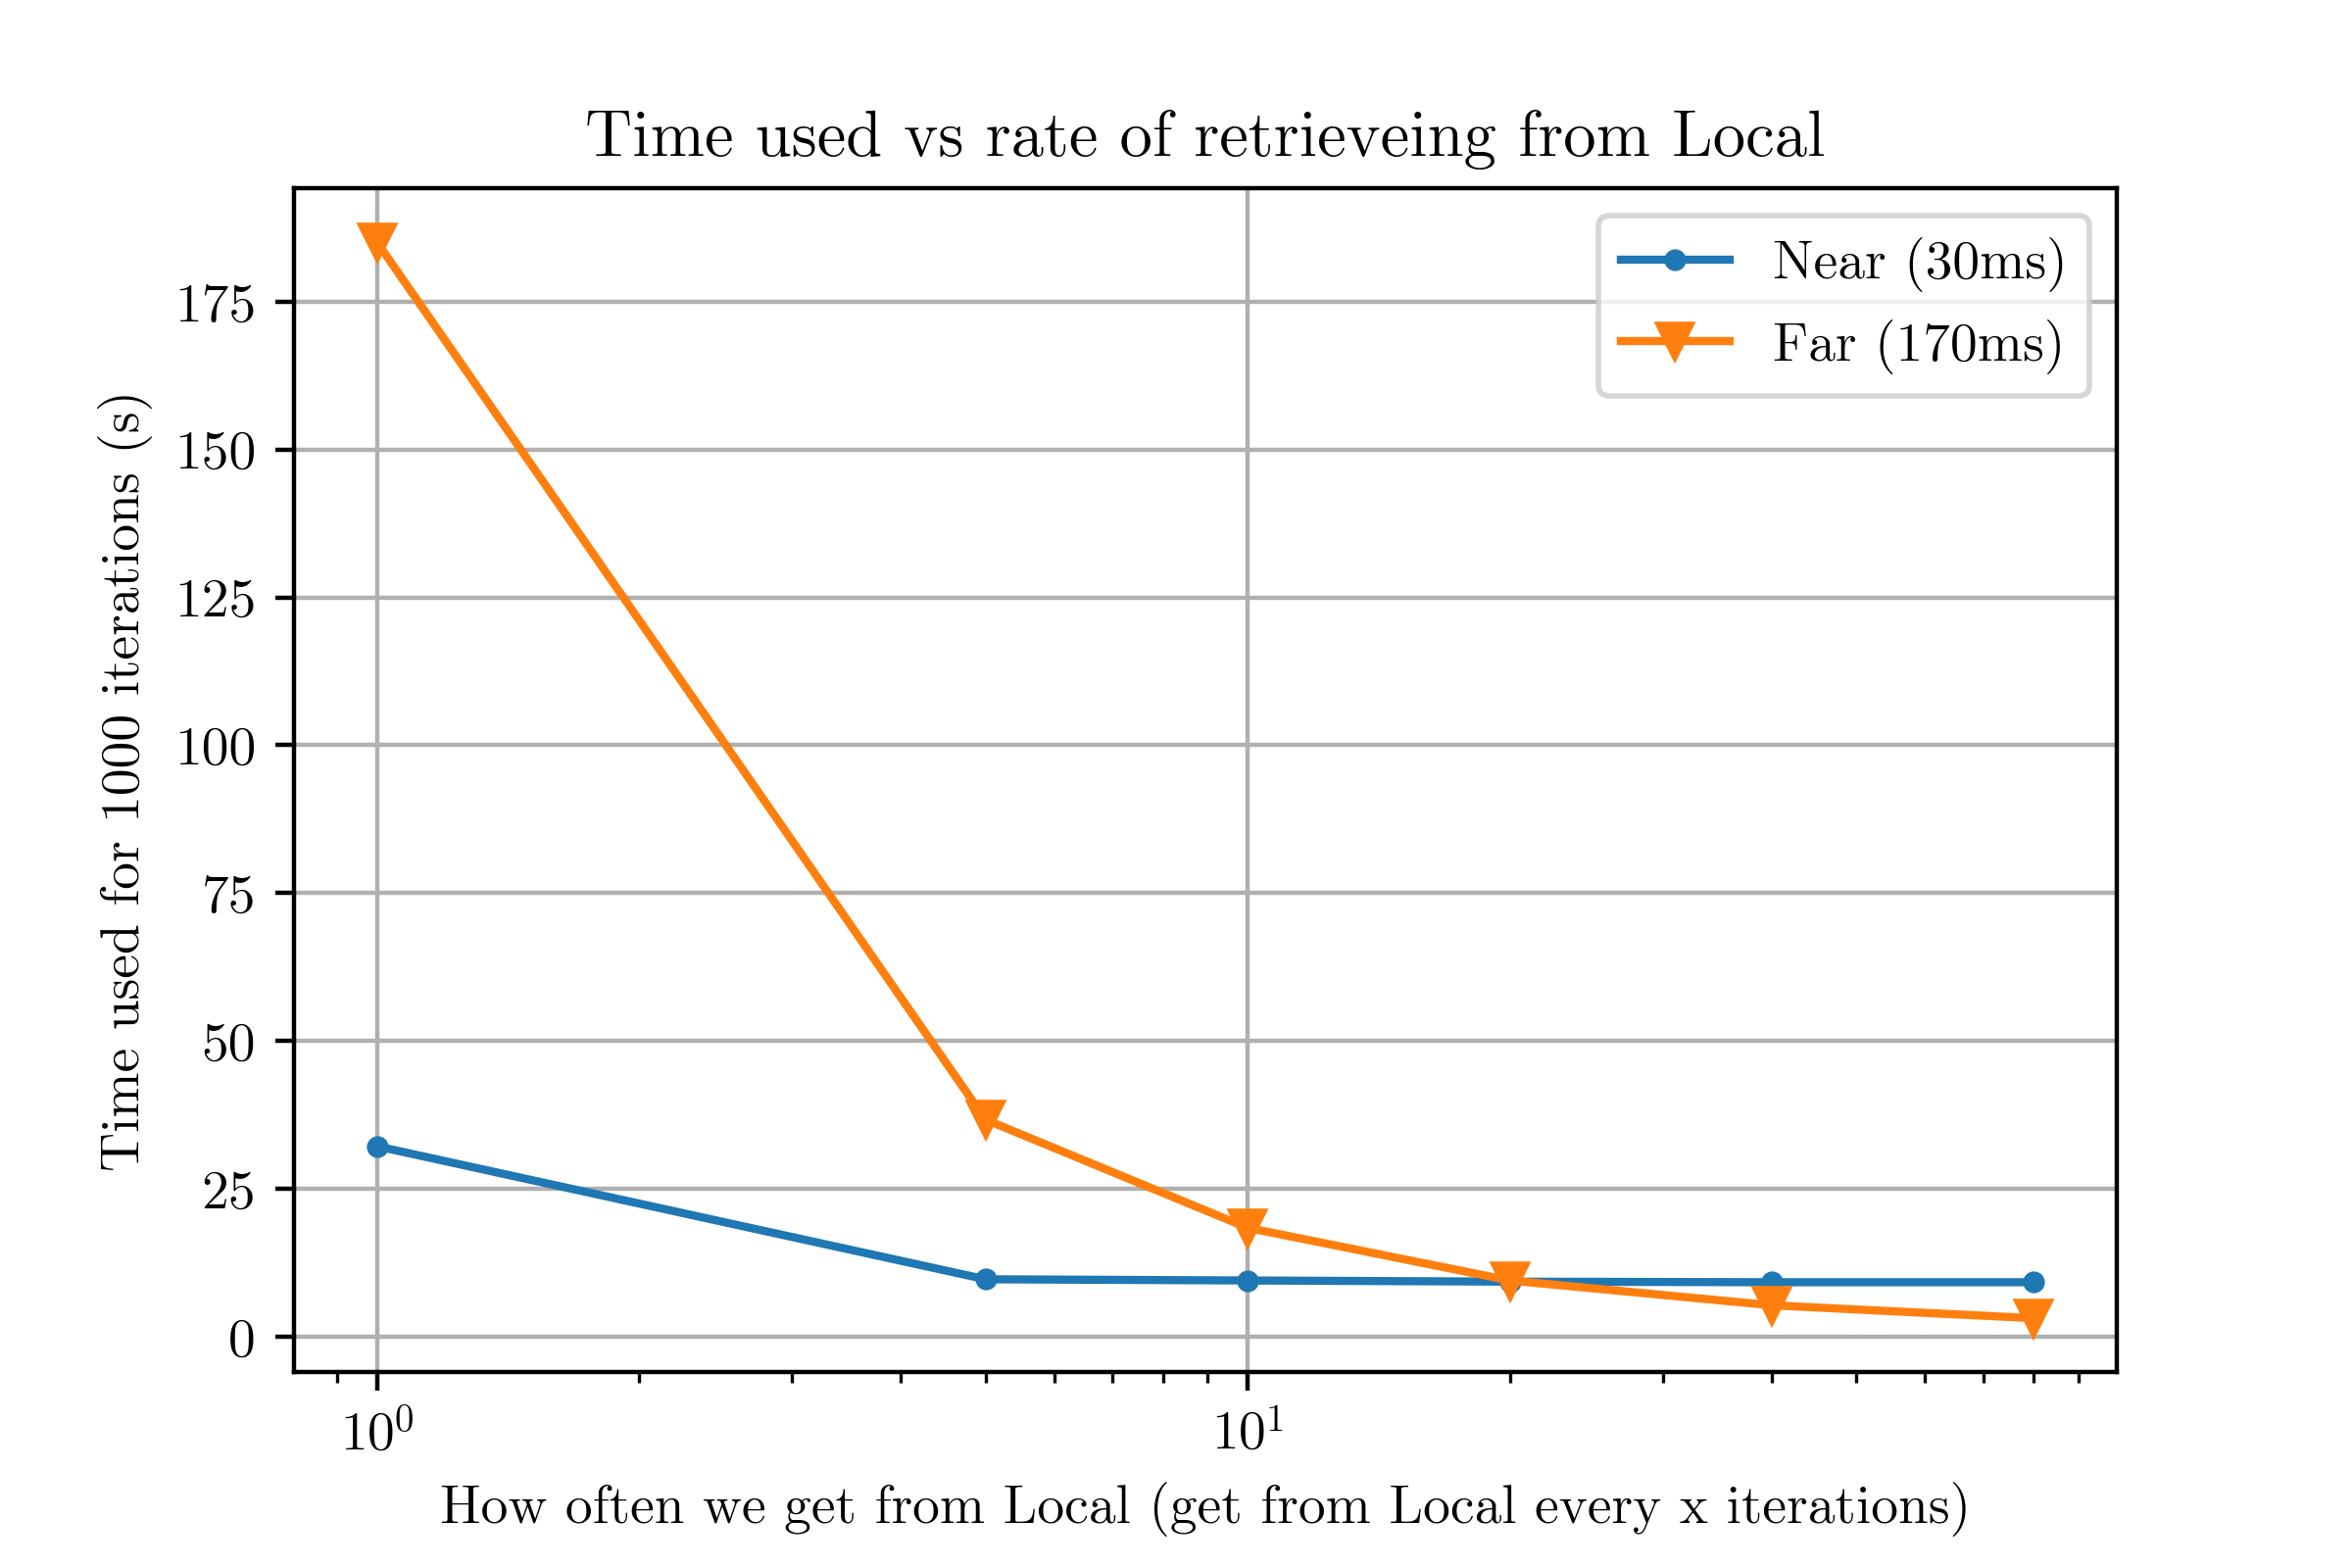
\includegraphics[scale=1]{chapters/evaluation/figures/times.png}
    \caption{Graph showing how interaction hurts. If x=10 then we get from Local every 10 iterations.}
    \label{fig:time_graph_near_far}
\end{figure}

Figure \ref{fig:time_graph_near_far} shows how latency affects the time used when you have to constantly get info from the mobile device (Local). If you constantly have to get info from the mobile device, the time to complete the whole task will be much slower. If you don't need to get info that often, then the Far server will yield better results as it has more computational power.


%Bar chart med som viser hvor stor andel av de forskjellige utregningene som består av calulation og latency

\begin{figure}[t]
    \centering
    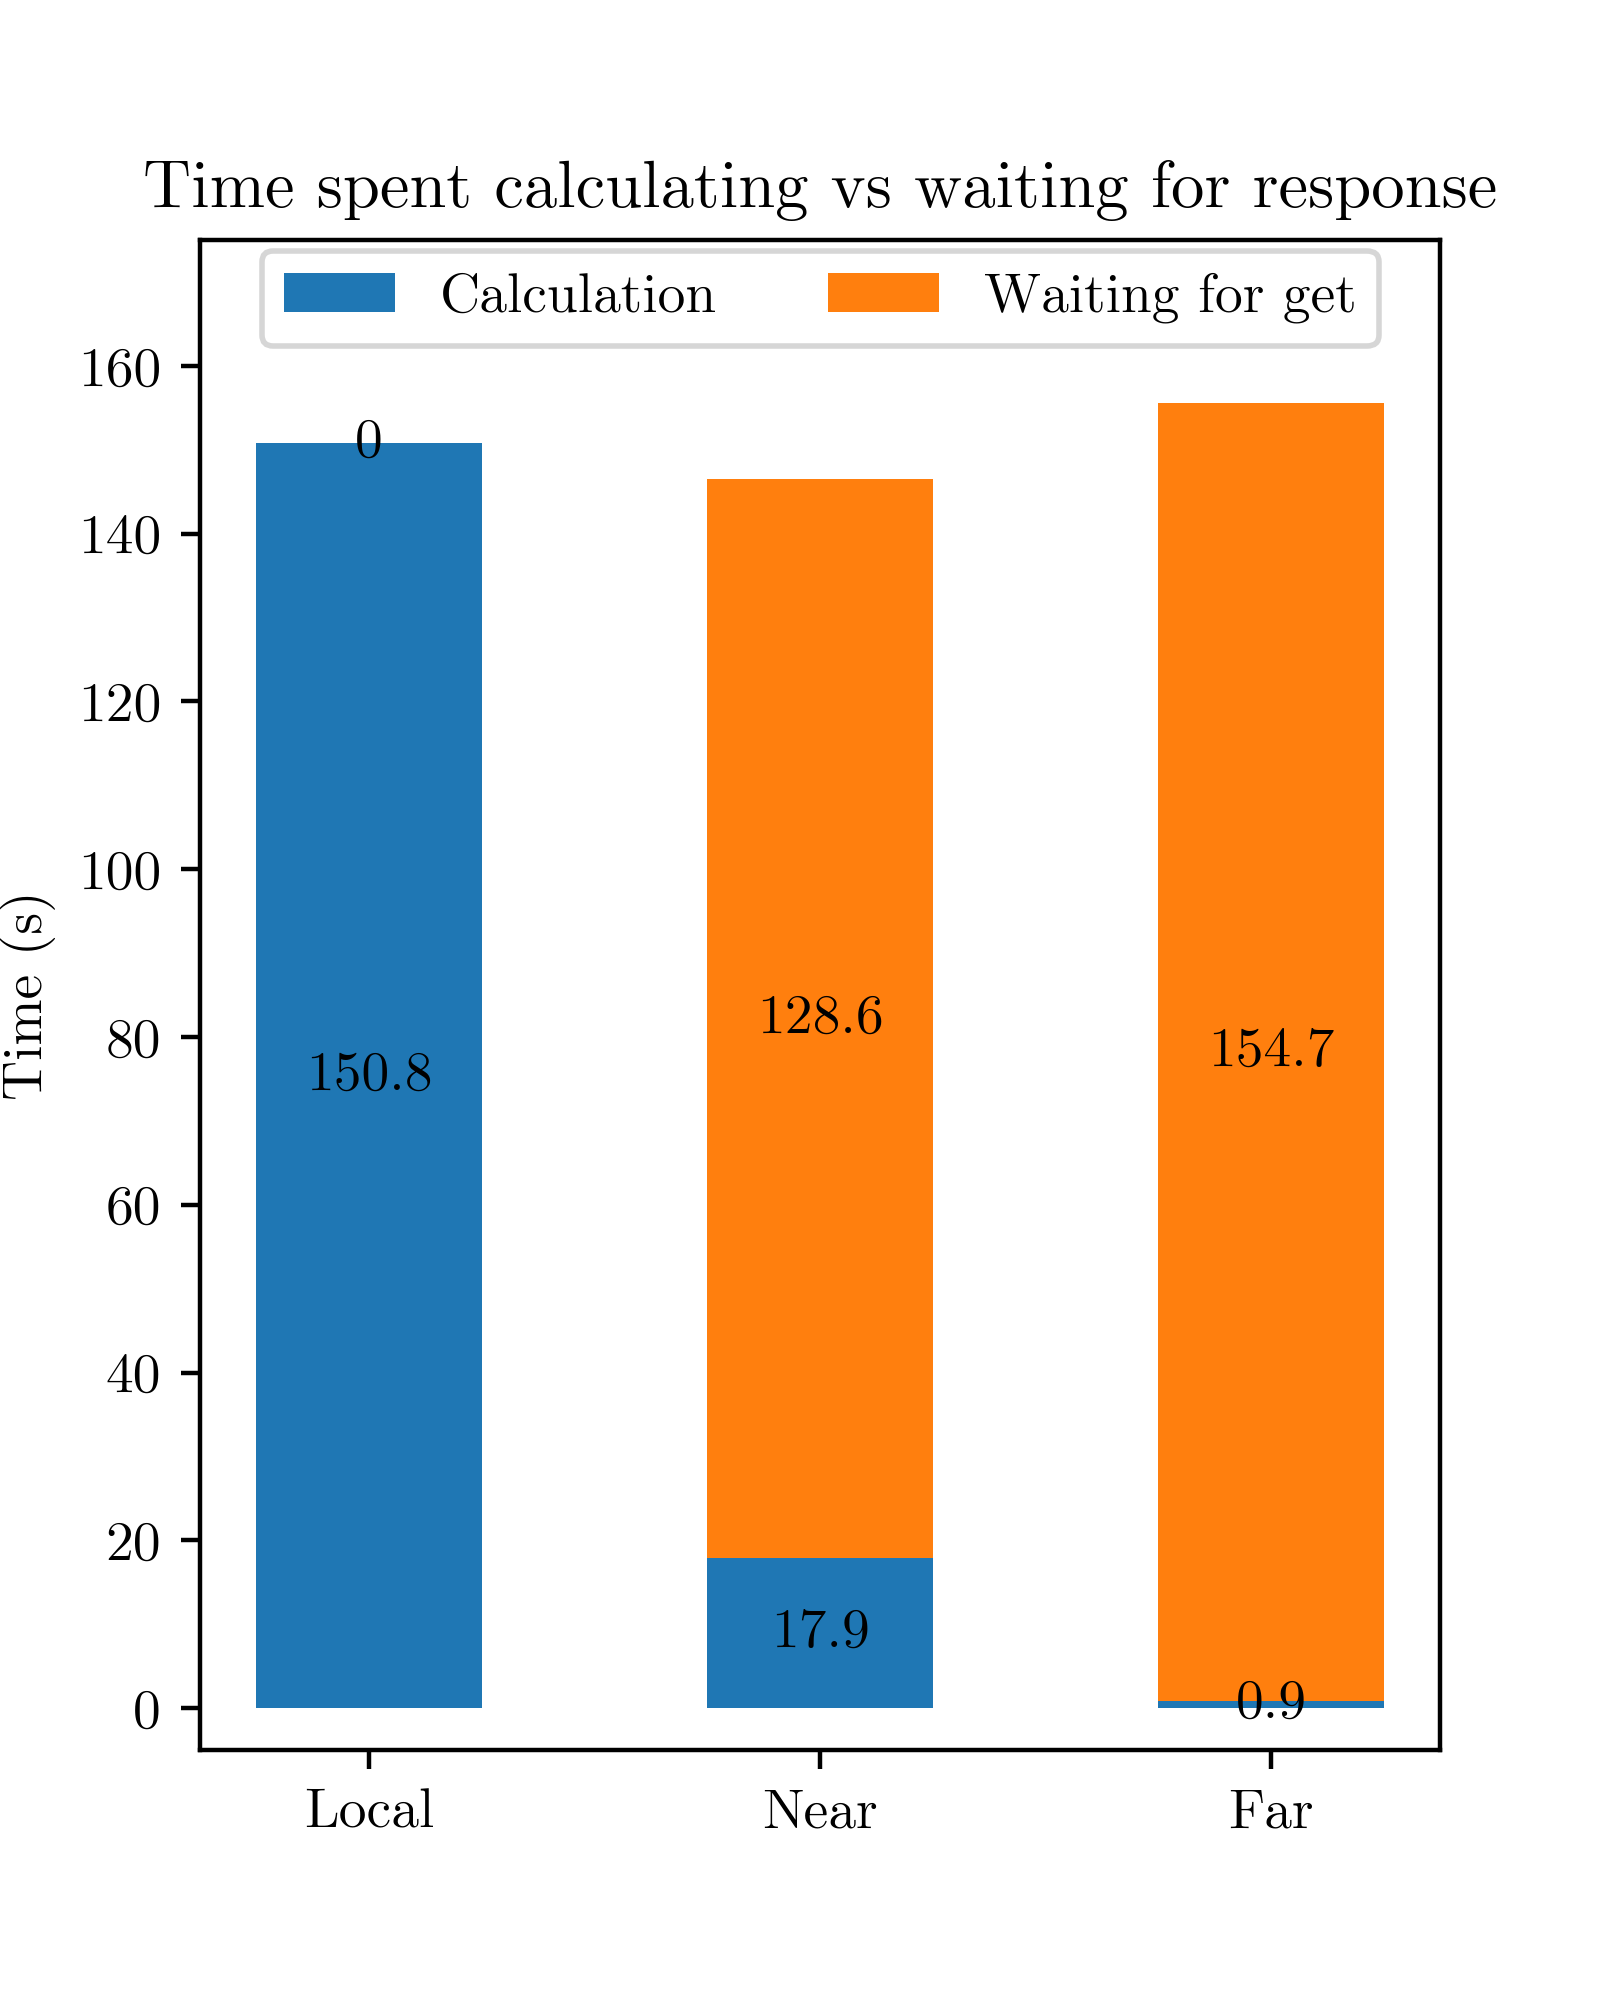
\includegraphics[scale=1]{chapters/evaluation/figures/bar_local_near_far_compare.png}
    \caption{bla}
    \label{fig:bar_local_near_far}
\end{figure}


\subsection{Characteristics}
%tabell? subsections? idk

%TODO
% Gjøre målinger med overføring av filer først. Finn data på bandwidth og pluss det på tiden.
% Gjøre målinger hvor det kreves mer samhandling mellom nodene. Vi må se latency!


%\cite{mach_mobile_2017} for hvor mye som skal offloades.!!!!
% test med 100% offload, 50% offload osv
%\begin{itemize}
 %   \item Easily scalable as we have the common interface. This makes it easy to add more vms to run more apps. So, its horizontally scalable?
%\end{itemize}







\section{Cloudlets}







\section{Amazon Cloudfront}
TODO: Warm up time for lambda.
\section{Summary}
TODO

\section{Comparison of the architectures}
TODO